%% -*- coding:utf-8 -*-

\section{Locality}
\label{Abschnitt-Diskussion-Lokalitaet}\label{sec-locality}

The\is{locality|(} question of local accessibility of information has been treated in various ways by the theories
discussed in this book. In the majority of theories, one tries to make information about the inner workings of phrases inaccessible
for adjacent or higher heads, that is, \emph{glaubt} `believe' in (\mex{1}) selects a sentential argument but it cannot ``look
inside'' this sentential argument.
\eal
\ex 
\gll Karl glaubt, dass morgen seine Schwester kommt.\\
	 Karl believes that tomorrow his sister comes\\
\glt `Karl believes that his sister is coming tomorrow.'
\ex 
\gll Karl glaubt, dass seine Schwester morgen kommt.\\
	 Karl believes that his sister tomorrow comes\\
\zl
Thus for example, \emph{glauben} cannot enforce that the subject of the verb has to begin with a consonant or that the complementizer
has to be combined with a verbal projection starting with an adjunct.
In Section~\ref{Abschnitt-Kopf}, we saw that it is a good idea to classify constituents in terms of their distribution and
independent of their internal structure. If we are  talking about an NP box, then it is not important what this NP box actually
contains. It is only of importance that a given head wants to be combined with an NP with a
particular case marking. This is called \emph{locality of selection}.

Various linguistic theories have tried to implement locality of selection. The simplest form of this implementation is shown by
phrase structure grammars of the kind discussed in Chapter~\ref{Kapitel-PSG}. The rule in (\ref{ditrans-schema}) on
page~\pageref{ditrans-schema}, repeated here as (\mex{1}), states that a ditransitive verb can occur with three noun phrases, each
with the relevant case:
\ea
\begin{tabular}[t]{@{}l@{ }l@{ }l}
S  & $\to$ & NP({Per1},{Num1},{nom}) \\
   &       & NP(Per2,Num2,{dat})\\
   &       & NP(Per3,Num3,{acc})\\
   &       & V({Per1},{Num1},ditransitive)\\
\end{tabular}
\z
Since the symbols for NPs do not have any further internal structure, the verb cannot require that there has to be a relative
clause in an NP, for example. The internal properties of the NP are not visible to the outside.
We have already seen in the discussion in Chapter~\ref{Kapitel-PSG}, however, that certain properties of phrases have to be outwardly
visible. This was the information that was written on the boxes themselves. For noun phrases, at least information about
person, number and case are required in order to correctly capture their relation to a head.
The gender value is important in German as well, since adverbial phrases such as \emph{einer nach
  dem anderen} `one after the other' have to agree in gender\is{gender} with the noun they refer to
(see example (\ref{Beispiel-einer-nach-dem-anderen}) on
page~\pageref{Beispiel-einer-nach-dem-anderen}). Apart from that, information about the length of
the noun phrases is required, in order to determine their order in a clause. Heavy constituents are normally ordered after lighter ones, and are also often
extraposed (cf.\ Behaghel's \textit{Gesetz der wachsenden Glieder}\is{Gesetz der wachsenden Glieder} `Law of increasing constituents' (\citeyear[\page
139]{Behaghel09}; \citeyear[\page 86]{Behaghel30})). 

Theories that strive to be as restrictive as possible with respect to locality therefore have to develop mechanisms that allow one to only
access information that is required to explain the distribution of constituents.
This is often achieved by projecting certain properties to the mother node of a phrase. In \xbart, the part of speech a head belongs to is
passed up to the maximal projection: if the head is an N, for example, then the maximal projection is an NP. In GPSG, HPSG and variants
of CxG, there are Head Feature Principles responsible for the projection of features. Head Feature Principles ensure that an entire group of
features, so"=called head features, are present on the maximal projection of a head.
Furthermore, every theory has to be capable of representing the fact that a constituent can lack one of its parts and this part is then realized via a long"=distance
dependency in another position in the clause.
As previously discussed on page~\pageref{Seite-Irishe-Komplementierer}, there are languages in which complementizers inflect depending on whether their
complement is missing a constituent or not. This means that this property must be somehow accessible. In GPSG, HPSG and variants of CxG, there are additional
groups of features that are present at every node between a filler and a gap in a long"=distance dependency.
In LFG, there is f"=structure\is{f"=structure} instead. Using Functional Uncertainty, one can look for the position in the f"=structure where a particular
constituent is missing. In \gbt, movement proceeds cyclically\is{cycle!transformational}, that is, an element is moved into the specifier of CP and can
be moved from there into the next highest CP. It is assumed in \gbt that heads can look inside their arguments, at least they can see the elements in the
specifier position. If complementizers can access the relevant specifier positions, then they can
determine whether something is missing from an embedded phrase or not. In \gbt, there was also an analysis of case
assignment in infinitive constructions in which the case"=assigning verb governs into the embedded
phrase and assigns case to the element in \mbox{SpecIP}. Figure~\ref{Abbildung-ECM} shows the
relevant structure taken from \citew[\page 170]{Haegeman94a-u}.
\begin{figure}
\centering
\begin{forest}
sn edges
[IP
	[NP
		[John]]
	[I$'$
		[I
			[-s]]
		[VP
			[V$'$
				[V
					[believe]]
				[IP
					[NP
						[him]]
					[I$'$
						[I
							[to]]
						[VP
							[V$'$
								[V
									[be]]
								[NP
									[a liar,triangle]]]]]]]]]]
\end{forest}
\caption{\label{Abbildung-ECM}Analysis of the AcI construction with \emph{Exceptional Case Marking}}
\end{figure}%
Since the Case Principle is formulated in such a way that only finite I can assign case to the subject
(cf. page~\pageref{Kasusprinzip-GB}), \emph{him} does not receive case from I. Instead, it is assumed that
the verb \emph{believe} assigns case to the subject of the embedded infinitive.

Verbs that can assign case across phrase boundaries are referred to as ECM verbs, where ECM stands for
\emph{Exceptional Case Marking}\is{Exceptional Case Marking (ECM)}. As the name suggests, this instance of case assignment into a phrase was viewed as an
exception. In newer versions of the theory (\eg \citealp[\page 120--123]{Kratzer96a}), all case assignment
is to specifier positions. For example, the Voice\is{category!functional!Voice} head in Figure~\vref{Abbildung-Kratzer} assigns
accusative to the DP in the specifier of VP.
\begin{figure}
\centering
\begin{forest}
sn edges
[VoiceP
	[DP
		[Mittie]]
	[Voice$'$
		[Voice
			[agent]]
		[VP
			[DP
				[the dog,triangle]]
			[V$'$
				[V
					[feed]]]]]]
\end{forest}
\caption{\label{Abbildung-Kratzer}Analysis of structures with a transitive verb following Kratzer}
\end{figure}%
Since the Voice head governs into the VP, case assignment to a run"=of"=the"=mill object in this theory
is an instance of exceptional case assignment as well. The same is true in Adger's version of
Minimalism, which was discussed in Chapter~\ref{chap-mp}: \citet{Adger2010a} argues that
his theory is more restrictive than LFG or HPSG since it is only one feature that can be selected by
a head, whereas in LFG and HPSG complex feature bundles are selected. However, the strength of
this kind of locality constraint is weakened by the operation Agree\is{Agree}, which allows for
nonlocal feature checking. As in Kratzer's proposal, case is assigned nonlocally by \littlev to
the object inside the VP (see Section~\ref{sec-case-mp}). 

Adger discusses PP arguments of verbs like \emph{depend} and notes that these verbs need specific
PPs, that is, the form of the preposition in the PP has to be selectable. While this is trivial in
Dependency Grammar, where the preposition is selected right away, the respective information is
projected in theories like HPSG and is then selectable at the PP node. However, this requires that
the governing verb can determine at least two properties of the selected element: its part of speech
and the form of the preposition. This is not possible in Adger's system and he left this for further
research. Of course it would be possible to assume an onP (a phrasal projection of \emph{on} that
has the category `on'). Similar solutions have been proposed in Minimalist theories (see
Section~\ref{sec-functional-projections-minimalism} on functional projections), but such a solution would obviously
miss the generalization that all prepositional phrases have something in common, which would not be
covered in a system with atomic categories that are word specific.


In theories such as LFG\indexlfg and HPSG\indexhpsg, case assignment takes place locally in constructions
such as those in (\mex{1}):

\eal
\ex John believes him to be a liar.
\ex 
\gll Ich halte ihn für einen Lügner.\\
	 I hold him for a.\acc{} liar\\
\glt `I take him to be a liar.'
\ex 
\gll Er scheint ein Lügner zu sein.\\
	 he seems a.\nom{} liar to be\\
\glt `He seems to be a liar.'	 
\ex 
\gll Er fischt den Teich leer.\\
	 he fishes the.\acc{} pond empty\\
\glt `He fishes (in) the pond (until it is) empty.'
\zl
Although \emph{him}, \emph{ihn} `him', \emph{er} `he' and \emph{den Teich} `the pond' are not semantic arguments of the finite verbs, they are syntactic arguments
(they are raised\is{raising}) and can therefore be assigned case locally. See \citew[\page 348--349 and Section~8.2]{Bresnan82c} and \citew[Section~3.5]{ps2}
for an analysis of raising in LFG\indexlfg and HPSG\indexhpsg respectively. See \citew{Meurers99b}, \citew{Prze99}, and
\citew[Section~17.4]{MuellerLehrbuch1} for case assignment in HPSG and for its interaction with raising.

There are various phenomena that are incompatible with strict locality and require the projection of at least some information.
For example, there are question tags\is{question tag} in English\il{English} that must match the subject of the clause with which
they are combined:
\eal
\ex She is very smart, isn't she / * he?
\ex They are very smart, aren't they?
\zl
\citet{BF99a}, \citet{FB2003a} therefore propose making information about agreement or the referential index of the subject\is{subject}
available on the sentence node.\footnote{
  See also \citew[\page 89]{SP91a-u}.
}
In \citet{Sag2007a}, all information about phonology, syntax and semantics of the subject is represented as the value of a feature \textsc{xarg}\isfeat{xarg} (\textsc{external argument}).
Here, \emph{external argument} does not stand for what it does in \gbt, but should be understood in a more general sense. For example, it makes the possessive pronoun
accessible on the node of the entire NP. \citet{Sag2007a} argues that this is needed to force coreference in English\il{English} idioms\is{idiom|(}:
\eal
\ex He$_i$ lost [his$_i$ / *her$_j$ marbles].
\ex They$_i$ kept/lost [their$_i$ / *our$_j$ cool].
\zl
The use of the \textsc{xarg} feature looks like an exact parallel to accessing the specifier position as we saw in the discussion of GB. However, Sag proposes that complements of prepositions
in Polish\is{Polish} are also made accessible by \textsc{xarg} since there are data suggesting that higher heads can access elements inside PPs \citep[Section~5.4.1.2]{Prze99b}.

In Section~\ref{sec-SbCxG} about Sign-based Construction Grammar, we already saw that a theory that only makes the reference to one
argument available on the highest node of a projection cannot provide an analysis for idioms of the
kind given in (\mex{1}). This is because the subject is made available with verbal heads, however,
it is the object that needs to be accessed in sentences such as (\mex{1}). This means that one has
to be able to formulate constraints affecting larger portions of syntactic structure.
\eal
\ex[]{\label{ex-ich-glaube-mich-tritt-ein-Pferd}
\gll Ich glaube, mich / \# dich tritt ein Pferd.\footnotemark\\
     I   believes me   {} {} you kicks a horse\\
\footnotetext{
  \citew[\page 311]{RS2009a}.
}
\glt `I am utterly surprised.'
}
\ex[]{
\gll Jonas glaubt, ihn  tritt ein Pferd.\footnotemark\\
     Jonas believes him kicks a horse\\
\footnotetext{
  \url{http://www.machandel-verlag.de/der-katzenschatz.html}, 06.07.2015.
}
\glt `Jonas is utterly surprised.'
}
\ex[\#]{
\gll Jonas glaubt, dich  tritt ein Pferd.\\
     Jonas believes you kicks a horse\\
\glt `Jonas believes that a horse kicks you.'
}
\zl
Theories of grammar with extended locality domains do not have any problems with this kind of data.\footnote{
Or more carefully put: they do not have any serious problems since the treatment of idioms in all their
many aspects is by no means trivial \citep{Sailer2000a}.
} An example for this kind of theory is TAG. In TAG, one can specify trees of exactly the right size \citep{Abeille88a,AS89a}.
All the material that is fixed in an idiom is simply determined in the elementary tree. Figure\vref{Abbildung-kick-the-bucket-TAG} shows
the tree for \emph{kick the bucket} as it is used in (\mex{1}a).
\eal
\ex The cowboys kicked the bucket.
\ex Cowboys often kick the bucket.
\ex He kicked the proverbial bucket.
\zl
\begin{figure}
\centering
\begin{forest}
tag
[S
	[NP$\downarrow$]
	[VP
		[V
			[kicked]]
		[NP
			[D
				[the]]
			[N
				[bucket]]]]]
\end{forest}
\caption{\label{Abbildung-kick-the-bucket-TAG}Elementary tree for \emph{kick the bucket}}
\end{figure}%
Since TAG trees can be split up by adjunction, it is possible to insert elements between the parts of an idiom as in (\mex{0}b,c) and thus
explain the flexibility of idioms with regard to adjunction and embedding.\footnote{
	Interestingly, variants of Embodied CxG are strikingly similar to TAG. The Ditransitive
        Construction that was discussed	on page~\pageref{CxG-Active-Ditransitive} allows for additional material to occur between the subject and the verb.
	
	The problems that arise for the semantics construction are also similar. \citet[\page
9]{AS89a} assume that the semantics of \emph{John kicked the proverbial bucket} is computed
from the parts \relation{John}, \relation{kick-the-bucket} and \relation{proverbial}, that is, the added modifiers
always have scope over the entire idiom. This is not adequate for all idioms \citep{FK96a}:
\ea
\gll Er band ihr einen großen Bären auf.\\
	 he tied her a big bear on\\
\glt `He pulled (a lot of) wool over her eyes.'
\z
In the idiom in (i), \emph{Bär} `bear' actually means `lie' and the adjective has to be interpreted accordingly.
The relevant tree should therefore contain nodes that contribute semantic information and also say something
about the composition of these features.

In the same way, when computing the semantics of noun phrases in TAG and Embodied Construction Grammar, one should bear in mind that the adjective
that is combined with a discontinuous NP Construction (see page~\pageref{CxG-DetNoun}) or an NP tree can have narrow scope over the noun
(\emph{all alleged murderers}).
} Depending on whether the lexical rules for the passive\is{passive} and long"=distance dependencies can be applied, the idiom can occur
in the relevant variants.

In cases where the entire idiom or parts of the idiom are fixed, it is possible to rule out adjunction to the nodes of the idiom
tree. Figure~\vref{Abbildung-take-into-account-TAG} shows a pertinent example from
\citet[\page 7]{AS89a}. The ban on adjunction\is{adjunction!ban} is marked by a subscript NA.
\begin{figure}
\centering
\begin{forest}
tag
[S
	[NP$\downarrow$]
	[VP
		[V
			[takes]]
		[NP$\downarrow$]
		[PP$_{{\mathrm{NA}}}$
			[P
				[into]]
			[NP$_{\mathrm{NA}}$
				[N$_{\mathrm{NA}}$
					[account]]]]]]
\end{forest}
\caption{\label{Abbildung-take-into-account-TAG}Elementary tree for \emph{take into account}}
\end{figure}%

The question that also arises for other theories is whether the efforts that have been made to enforce locality should be abandoned altogether.
In our box model in Section~\ref{Abschnitt-Kopf}, this would mean that all boxes were transparent. Since plastic boxes do not allow
all of the light through, objects contained in multiple boxes cannot be seen as clearly as those in the top"=most box (the path
of Functional Uncertainty\is{functional uncertainty} is longer). This is parallel to a suggestion made by
\citet{KF99a} in CxG\indexcxg. Kay and Fillmore explicitly represent all the information about the internal structure of a phrase on the mother
node and therefore have no locality restrictions at all in their theory. In principle, one can
motivate this kind of theory in parallel to the argumentation in Chapter~\ref{Abschnitt-Generative-Kapazitaet}. The argument
there made reference to the complexity of the grammatical formalism: the kind of complexity that the
language of description has is unimportant, it is only important what one does with it. In the same way, one can say that regardless of what kind of information
is  in principle accessible, it is not accessed if this is not permitted. This was the approach taken by \citet[\page
143--145]{ps}.

It\label{page-Bender-Wambaya-two} is also possible to assume a world in which all the boxes contain transparent areas where it is possible to see parts of their contents.
This is more or less the LFG world\indexlfg: the information about all levels of embedding contained in the f"=structure\is{f"=structure} is
visible to both the inside and the outside. We have already discussed Nordlinger's \citeyearpar{Nordlinger98a-u} LFG analysis of Wambaya\il{Wambaya} 
on page~\pageref{Seite-Bender-Wambaya}.
In Wambaya, words that form part of a noun phrase can be distributed throughout the clause. For example, an adjective that refers to a noun
can occur in a separate position from it. Nordlinger models this by assuming that an adjective can make reference to an argument in the f"=structure
and then agrees with it in terms of case, number and gender. \citet{Bender2008a} has shown that this analysis can be transferred to HPSG\indexhpsg:
instead of no longer representing an argument on the mother node after it has been combined with a head, simply marking the argument as realized
allows us to keep it in the representation (\citealp{Meurers99b}; \citealp{Prze99};
\citealp[Section~17.4]{MuellerLehrbuch1}). Detmar Meurers\aimention{Walt Detmar
  Meurers} compares both of these HPSG approaches to different ways of working through a shopping list: in the standard approach taken by \citet{ps2},
one tears away parts of the shopping list once the relevant item has been found. In the other case, the relevant item on the list is crossed out.
At the end of the shopping trip, one ends up with a list of what has been bought as well as the items themselves.
  
I have proposed the crossing"=out analysis for depictive predicates\is{depictive predicate|(} in German and English 
\citep{Mueller2004c,Mueller2008a}. Depictive predicates say something about the state of a person or object during the event
expressed by a verb:
\eal
\ex 
\gll Er sah sie nackt.\footnotemark\\
	 he saw her naked\\
\footnotetext{
  \citew[\page 94]{Haider85b}.
}
\ex He saw her naked.
\zl
In (\mex{0}), the depictive adjective can either refer to the subject or the object. However, there is a strong preference for readings where
the antecedent noun precedes the depictive predicate
\citep[\page 208]{Loetscher85}. Figure~\vref{anal-er-die-frau-nackt-sieht} shows analyses for the
sentences in (\mex{1}):
\eal
\ex 
\gll dass er$_i$ die Äpfel$_j$ ungewaschen$_{i/j}$ isst\\
	 that he the apples unwashed eats\\
\glt `that he eats the apples unwashed'
\ex 
\gll dass er$_i$ ungewaschen$_{i/*j}$ die Äpfel$_j$ isst\\
	 that he unwashed the apples eats\\
\glt `that he eats the apples (while he is) unwashed'
\zl
\begin{figure}
%\hfill
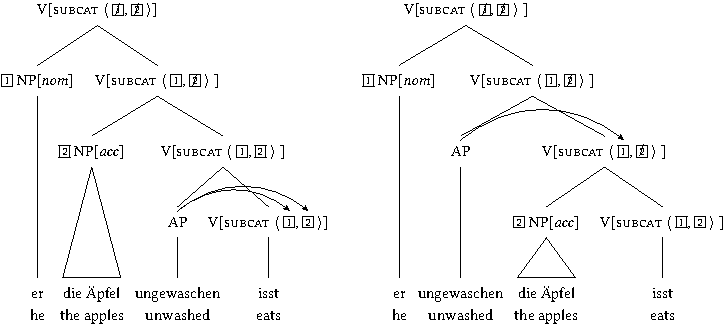
\includegraphics[width=\textwidth]{Figures/depictives-lsp-cropped.pdf}
%%  \resizebox{\linewidth}{!}{%
%% \begin{forest}
%% sn edges, for tree={l sep= 6ex}
%% [V{[\subcat \sliste{ \spirit{1}, \spirit{2} }]}
%% 	[\ibox{1} NP{[\textit{nom}]}
%% 		[er;he]]
%% 	[V{[\subcat \sliste{ \ibox{1}, \spirit{2} } ]}
%% 		[\ibox{2} NP{[\textit{acc}]}
%% 			[die Äpfel;the apples,triangle]]
%% 		[V{[\subcat \sliste{ \ibox{1}, \ibox{2} } ]}
%% 			[\subnode{ap1}{AP}
%% 				[ungewaschen;unwashed]]
%% 			[V{[\subcat \sliste{ \subnode{arg11}{\ibox{1}}, \subnode{arg12}{\ibox{2}} }]}
%% 				[isst;eats]]]]]
%% \end{forest}
%% \hspace{1em}
%% \begin{forest}
%% sn edges, for tree={l sep= 6ex}
%% [V{[\subcat \sliste{ \spirit{1}, \spirit{2} } ]}
%% 	[\ibox{1} NP{[\textit{nom}]}
%% 		[er;he]]
%% 	[V{[\subcat \sliste{ \ibox{1}, \spirit{2} } ]}
%% 		[\subnode{ap2}{AP}
%% 			[ungewaschen;unwashed]]
%% 		[V{[\subcat \sliste{ \subnode{arg21}{\ibox{1}}, \spirit{2} } ]}
%% 			[\ibox{2} NP{[\textit{acc}]}
%% 				[die Äpfel;the apples,triangle]]
%% 			[V{[\subcat \sliste{ \ibox{1}, \ibox{2} } ]}
%% 				[isst;eats]]]]]
%% \end{forest}
%% % This has to be inside of the scaling
%%     %% \begin{tikzpicture}[overlay,remember picture]
%%     %% %% this works with tikzmark
%%     %% \draw[->, bend angle=40, bend left] ($(pic cs:ap1)+(1ex,2ex)$) to($(pic cs:arg11)+(1ex,2.5ex)$);
%%     %% \draw[->, bend angle=40, bend left] ($(pic cs:ap1)+(1ex,2ex)$) to($(pic cs:arg12)+(1ex,2.5ex)$); % 1ex links, 2ex hoch
%%     %% %
%%     %% \draw[->, bend angle=40, bend left] ($(pic cs:ap2)+(1ex,2ex)$) to($(pic cs:arg21)+(1ex,2.5ex)$);
%%     %% \end{tikzpicture}
%% % somehow it stopped working
%% %% this used to work with subnode in texlive 2013 but is broken now
%% \begin{tikzpicture}[overlay,remember picture] 
%% \draw[->, bend angle=40, bend left] (ap1.north) to (arg11.north);
%% \draw[->, bend angle=40, bend left] (ap1.north) to (arg12.north); 
%% %
%% \draw[->, bend angle=40, bend left] (ap2.north) to (arg21.north);
%% \end{tikzpicture}
%}
%\hfill\mbox{}
\caption{Analysis of \emph{dass er die Äpfel ungewaschen isst} `that he the apples unwashed eats' and \emph{dass er ungewaschen die
    Äpfel isst} `that he unwashed the apples eat'}\label{anal-er-die-frau-nackt-sieht}
\end{figure}%
Arguments that have been realized are still represented on the upper nodes, however, they are crossed"=out and thereby marked as ``realized''.
In German, this preference for the antecedent noun can be captured by assuming a restriction that states that the antecedent noun must not yet have been
realized.

It is commonly assumed for English\il{English} that adjuncts are combined with a VP.
\eal
\ex John [[\sub{VP} ate the apples$_i$] unwashed$_i$].
\ex You can't [[\sub{VP} give them$_i$ injections] unconscious$_i$].\footnote{
\citew[\page 17]{Simpson2003a}.
}
\zl
In approaches where the arguments of the verb are accessible at the VP node, it is possible to establish a relation between
the depictive predicate and an argument although the antecedent noun is inside the VP.
English differs from German in that depictives can refer to both realized (\emph{them} in (\mex{0}b))
and unrealized (\emph{you} in (\mex{0}b)) arguments.

\citet[\page 560]{Higginbotham85a} and \citet{Winkler97a} have proposed corresponding non"=cancellation approaches in \gbt.
There are also parallel suggestions in Minimalist theories: checked features are not deleted, but instead marked as already
checked \citep[\page 14]{Stabler2010b}. However, these features are still viewed as inaccessible.\label{page-non-cancellation-end}

Depending on how detailed the projected information is, it can be possible to see adjuncts and argument in embedded structures as well as their
phonological, syntactic and semantic properties. In the CxG variant proposed by Kay and Fillmore, all information is available. In LFG,
information about grammatical function, case and similar properties is accessible. However, the part of speech is not contained in the f"=structure.
If the part of speech does not stand in a one"=to"=one relation to grammatical function, it cannot be restricted using selection via f"=structure.
Nor is phonological information represented completely in the f"=structure. If the analysis of idioms requires nonlocal access to phonological
information or part of speech, then this has to be explicitly encoded in the f"=structure (see \citew[\page 46--50]{Bresnan82a} for more on idioms). 

In the HPSG variant that I adopt, only information about arguments is projected. Since arguments are always represented by descriptions of type
\type{synsem}, no information about their phonological realization is present. However, there are daughters in the structure so that it is still
possible to formulate restrictions for idioms as in TAG or Construction Grammar (see \citew{RS2009a}
for an analysis of the `horse' example in (\ref{ex-ich-glaube-mich-tritt-ein-Pferd})).
This may seem somewhat like overkill: although we already have the tree structure, we are still projecting information about arguments
that have already been realized (unfortunately these also contain information about their arguments and so on). At this point, one could be inclined
to prefer TAG or LFG since these theories only make use of one extension of locality: TAG uses trees
of arbitrary or rather exactly the necessary size and LFG makes reference to a complete
f"=structure. However, things are not quite that simple: if one wants to create a relation to an
argument when adjoining a depictive predicate in TAG, then one requires a list of
possible antecedents. Syntactic factors (\eg reference to dative vs.\ accusative noun phrases, to argument vs.\ adjuncts,
coordination of verbs vs.\ nouns) play a role in determining the referent noun, this cannot be reduced to semantic relations.
Similarly, there are considerably different restrictions for different kinds of idioms and these cannot all be formulated in terms of restrictions
on f"=structure since f"=structure does not contain information about parts of speech.\is{depictive predicate|)}

One should bear in mind that some phenomena require reference to larger portions of structure. The majority of phenomena can be treated in terms of head
domains and extended head domains, however, there are idioms that go beyond the sentence level. Every theory has to account for this somehow.
\is{locality|)}\is{idiom|)}



%      <!-- Local IspellDict: en_US-w_accents -->
